\newpage
\section{Zadanie 2}

\subsection{Opis zadania}

Dana jest funkcja
\[
Y = (A + B) \cdot \overline{C}.
\]
Wyjście załącza się, gdy jest $A$ albo $B$, i tylko pod warunkiem, że $C$ stoi w zerze. Jedynka na $C$ gasi $Y$ niezależnie od pozostałych dwóch wejść. $A$ i $B$ są równorzędne: każde z nich samo otwiera gałąź sumy.

\subsection{Wejścia i wyjścia}

Adresy są te same co w zadaniu~1. Inna jest rola I3: w drabince stoi jako styk zanegowany, nie jako osobna gałąź sumy.

\begin{table}[H]
    \centering
    \caption{Wejścia i wyjścia zadania 2}
    \label{tab:z2-io}
    \begin{tabular}{|l|l|p{8.2cm}|}
        \hline
        \textbf{Sygnał} & \textbf{Adres} & \textbf{Rola} \\
        \hline
        $A$ & I1 & pierwsza gałąź sumy \\
        \hline
        $B$ & I2 & druga gałąź sumy \\
        \hline
        $C$ & I3 & styk zanegowany, blokuje $Y$ \\
        \hline
        $Y$ & Q1 & wyjście \\
        \hline
    \end{tabular}
\end{table}

\subsection{Tablica prawdy}

Jedynka wypada tylko w trzech wierszach i wszystkie mają $C = 0$. Przy $C = 1$ kolumna $Y$ jest pusta, także wtedy, gdy $A$ i $B$ są jednocześnie załączone.

\begin{table}[H]
    \centering
    \caption{Tablica prawdy funkcji $Y = (A + B) \cdot \overline{C}$}
    \label{tab:z2-prawda}
    \begin{tabular}{|c|c|c|c|}
        \hline
        $A$ & $B$ & $C$ & $Y$ \\
        \hline
        0 & 0 & 0 & 0 \\
        \hline
        0 & 0 & 1 & 0 \\
        \hline
        0 & 1 & 0 & 1 \\
        \hline
        0 & 1 & 1 & 0 \\
        \hline
        1 & 0 & 0 & 1 \\
        \hline
        1 & 0 & 1 & 0 \\
        \hline
        1 & 1 & 0 & 1 \\
        \hline
        1 & 1 & 1 & 0 \\
        \hline
    \end{tabular}
\end{table}

\subsection{Funkcja logiczna}

Trzy wiersze z jedynką dają

\[
Y = \overline{A}\,B\,\overline{C} + A\,\overline{B}\,\overline{C} + A\,B\,\overline{C}.
\]

W każdym iloczynie jest $\overline{C}$. Przy $A = 0$ i $B = 0$ suma jest pusta, co zgadza się z dwoma pierwszymi wierszami tablicy~\ref{tab:z2-prawda}.

\subsection{Minimalizacja}

$\overline{C}$ wychodzi przed nawias:

\[
Y = \overline{C}\,(\overline{A}\,B + A\,\overline{B} + A\,B).
\]

W nawiasie $A\,\overline{B} + A\,B = A$ oraz $\overline{A}\,B + A\,B = B$, więc zostaje $A + B$:

\[
Y = (A + B) \cdot \overline{C}.
\]

Ta sama funkcja w postaci sumy iloczynów to $Y = A\,\overline{C} + B\,\overline{C}$. Obie postaci są minimalne, licząc inaczej: pierwsza ma jedną negację wspólną dla obu sygnałów, druga powtarza $\overline{C}$ w każdym iloczynie. Na sterownik wzięliśmy postać z nawiasem, bo wtedy styk zanegowany występuje raz, za węzłem, a nie w każdej gałęzi.

\subsection{Schemat logiczny}

$A$ i $B$ wchodzą na OR. $C$ przechodzi przez NOT i dopiero zanegowane spotyka się z sumą na bramce AND. Kreska nad $C$ jest bąbelkiem na wyjściu NOT, a nie osobnym sygnałem podanym z zewnątrz.

\begin{figure}[H]
    \centering
    \begin{circuitikz}[thick, font=\small]
        \node[or port] (ab) at (0,0.85) {};
        \node[not port] (nc) at (0.15,-1.25) {};
        \node[and port] (wy) at (3.7,0) {};
        \draw (ab.in 1) -- ++(-1.15,0) node[left] {$A$};
        \draw (ab.in 2) -- ++(-1.15,0) node[left] {$B$};
        \draw (ab.out) -- ++(0.45,0) |- (wy.in 1);
        \draw (nc.in) -- ++(-1.3,0) node[left] {$C$};
        \draw (nc.out) -- ++(0.55,0) |- (wy.in 2);
        \draw (wy.out) -- ++(0.85,0) node[right] {$Y$};
    \end{circuitikz}
    \caption{Schemat logiczny $Y = (A + B) \cdot \overline{C}$}
    \label{fig:z2-bramki}
\end{figure}

\subsection{Program PLC}

Na rys.~\ref{fig:z2-drabinka} styki I1 i I2 stoją równolegle. Za wspólnym węzłem jest zanegowany I3 i cewka Q1. Gałąź równoległa robi sumę $A + B$, styk z kreską przepuszcza ją dalej tylko przy $C = 0$.

\begin{figure}[H]
    \centering
    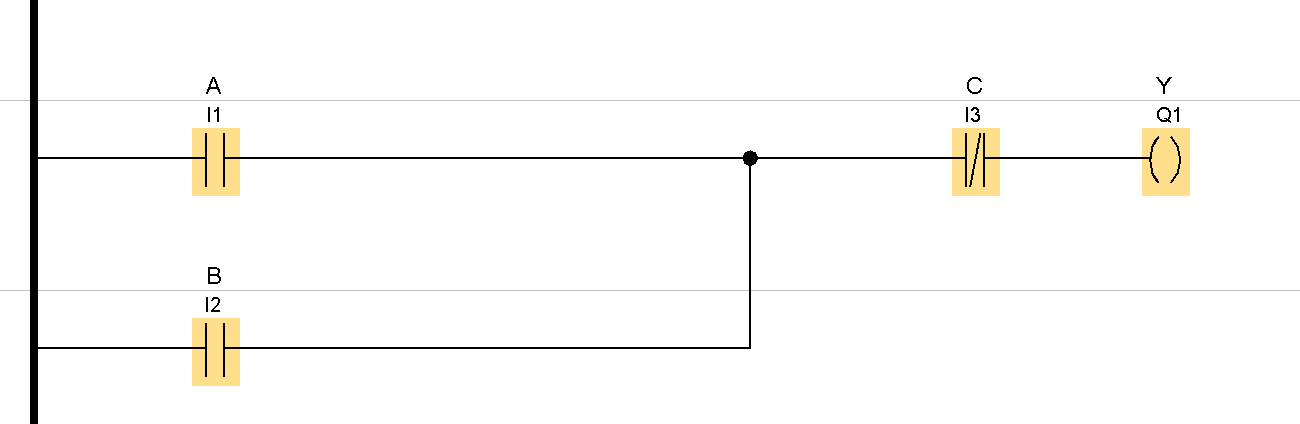
\includegraphics[width=0.88\textwidth]{rys/zad2/2_1_schemat.png}
    \caption{Drabinka zadania 2. I3 jest stykiem zanegowanym}
    \label{fig:z2-drabinka}
\end{figure}

Trzy stany z symulacji rozdzielają tę funkcję na części. Samo $B$ przy $C = 0$ załącza Q1, choć $A$ jest zerem (rys.~\ref{fig:z2-stany}a). Samo $A$ przy $C = 0$ robi to samo (rys.~\ref{fig:z2-stany}b). Gdy $A$ i $B$ są jedynkami, a do tego dojdzie $C = 1$, żarówka gaśnie: suma jest spełniona, ale styk zanegowany ją odcina (rys.~\ref{fig:z2-stany}c).

\begin{figure}[H]
    \centering
    \begin{subfigure}{\textwidth}
        \centering
        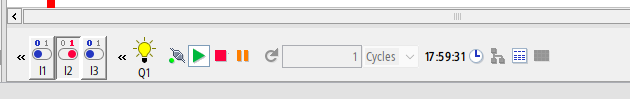
\includegraphics[width=0.70\textwidth]{rys/zad2/2_2_stan.png}
        \caption{$A = 0$, $B = 1$, $C = 0$, Q1 załączone}
    \end{subfigure}

    \vspace{0.4em}
    \begin{subfigure}{\textwidth}
        \centering
        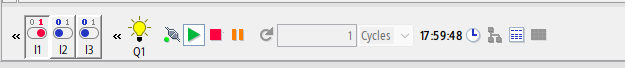
\includegraphics[width=0.70\textwidth]{rys/zad2/2_3stan.png}
        \caption{$A = 1$, $B = 0$, $C = 0$, Q1 załączone}
    \end{subfigure}

    \vspace{0.4em}
    \begin{subfigure}{\textwidth}
        \centering
        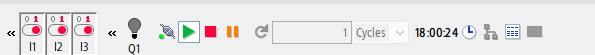
\includegraphics[width=0.70\textwidth]{rys/zad2/2_4stan.png}
        \caption{$A = 1$, $B = 1$, $C = 1$, Q1 zgaszone}
    \end{subfigure}
    \caption{Symulacja zadania 2}
    \label{fig:z2-stany}
\end{figure}
